\documentclass[titlepage,11pt]{article}
\usepackage{comment}
\usepackage{enumitem}
\usepackage{transparent} % Untuk transparansi gambar
\usepackage{listings}
\usepackage{amsmath}
\usepackage{graphicx}
\usepackage[font=small,labelfont=bf]{caption}
\usepackage[bahasa]{babel}
\usepackage{float}
\usepackage{verbatim}
\usepackage{graphicx,tabularx,multirow}
\usepackage{xcolor}
\usepackage[onehalfspacing]{setspace}
\usepackage[
	allcolors=visigrey,
	colorlinks=true,
]{hyperref}
\usepackage[a4paper,left=2cm,right=2cm]{geometry}
% Pengaturan kutipan artikel
\usepackage[style=ieee, backend=biber]{biblatex}
%Code listing style pak akok
\definecolor{codegreen}{rgb}{0,0.6,0}
\definecolor{codegray}{rgb}{0.5,0.5,0.5}
\definecolor{codepurple}{rgb}{0.58,0,0.82}
\definecolor{backcolour}{rgb}{0.95,0.95,0.92}

\usepackage{eso-pic} % Untuk menambahkan elemen ke seluruh halaman

\newcommand\BackgroundPic{
  \put(0,0){
    \parbox[b][\paperheight]{\paperwidth}{
      \vfill
      \centering
      \transparent{0.1}
      \includegraphics[width=0.4\paperwidth,keepaspectratio]{miot.png}
      \vfill
    }
  }
}

\newcommand\BackgroundAllPages{ \AddToShipoutPicture*{\BackgroundPic} }
\newcommand\BackgroundNone{ \ClearShipoutPicture } % hilangkan background

\lstdefinestyle{mystyle}{
	backgroundcolor=\color{backcolour}, commentstyle=\color{codegreen},
	keywordstyle=\color{magenta},
	numberstyle=\small\color{codegray},
	stringstyle=\color{codepurple},
	basicstyle=\ttfamily\footnotesize,
	breakatwhitespace=false,         
	breaklines=true,                 
	captionpos=t,                    
	keepspaces=true,                 
	numbers=left,                    
	numbersep=5pt,                  
	showspaces=false,                
	showstringspaces=false,
	showtabs=false,           
	frame = single,
	tabsize=2
}
\lstset{style=mystyle}

\definecolor{visigrey}{rgb}{.1,.15,.15}
\geometry{top=1cm,bottom=.5cm}
\savegeometry{titlepage}
\geometry{top=2cm,bottom=2cm}
\savegeometry{main}

\def\bspace{\(\qquad\qquad\qquad\)}
\usepackage[T1]{fontenc}
\usepackage[utf8]{inputenc}
\usepackage{tgheros}
\renewcommand*\familydefault{\sfdefault}

\setcounter{tocdepth}{6}

\def\autor{Laboratorium }
\def\lab{Multimedia dan Internet of Things}
\def\departemen{Departemen Teknik Komputer}
\def\institut{Institut Teknologi Sepuluh Nopember}
\def\praktikum{Laporan Sementara \\ Praktikum Jaringan Komputer}
\def\nama{Bintang Narindra Putra Pratama - 5024231038}
% Ubah Judul sesuai dengan modul
\def\judul{Wireless LAN dan Ubiquitous}
\def\tanggal{2025}
\begin{document}
% Ubah Bahasa sesuai dengan keinginan
\selectlanguage{bahasa}

\BackgroundNone
\def\headingtype{\bf \small}
\loadgeometry{titlepage}

\begin{titlepage}
	\centering
	\begin{tabularx}{\textwidth}{l@{\hskip 0pt}lX}
		\raisebox{-0.5\height}{
\includegraphics[width=3cm]{Cover/img/logodepart.png}} 
		& \raisebox{-0.5\height}{\includegraphics[width=3cm]{Cover/img/miot.png}} 
		& \raggedleft
	\hfill
	\begin{minipage}{0.5\textwidth}
		\raggedleft
		{\emph{\headingtype \autor}} \\[-2pt]
		{\headingtype \lab} \\[-2pt]
		{\headingtype \departemen} \\[-2pt]
		{\headingtype \emph{\institut}}
	\end{minipage}

	\vspace{5cm}
	\end{tabularx}
	
	\vspace{5cm}
	{\Huge \bf \praktikum \par}
	
	\vspace{2cm}
	{\LARGE \bf \judul \par}
	
	\vspace{2cm}
	{\Large \nama \par}
	
	\vfill
	{\Large \tanggal \par}
	
	\vfill
	
\includegraphics[width=\textwidth]{Cover/img/footer.png}
\end{titlepage}

\loadgeometry{main}


\BackgroundAllPages
% Pilih Modul yang akan di build
\section{Pendahuluan}
\subsection{Latar Belakang}
Seiring perkembangan zaman, koneksi jaringan komputer tidak lagi terbatas pada koneksi secara fisik dengan menggunakan kabel dengan munculnya teknologi wireless(nirkabel). Dengan teknologi ini kita dapat melakukan pertukaran informasi pada jarak yang lebih jauh dan tanpa perlu lagi membuat sebuah jaringan yang rumit. Contoh nyata dari teknologi wireless ini adalah WiFi dan Bluetooth. Selain itu, saat ini juga sedang berkembang teknologi ubiquitous computing yang membuat perangkat komputer hadir disetiap aktivitas kehidupan seperti sensor, smartphone, perangkat IoT, wearable device seperti smartwatch, dan sebagainya yang memungkinkan kita untuk mengakses informasi tanpa perlu perangkat komputer yang sesungguhnya. Teknologi ubiquitous computing ini sangat bergantung pada jaringan wireless untuk memungkinkan perangkat-perangkatnya tetap "tidak terlihat" oleh manusia. Dengan demikian praktikum tentang wireless LAN dan Ubiquitous ini sangat penting untuk meningkatkan kemampuan mahasiswa tentang konfigurasi jaringan wireless agar dapat membangun sistem jaringan yang responsif, adaptif, dan tersedia kapan saja.

\subsection{Dasar Teori}
Jaringan Wireless atau Jaringan Nirkabel adalah pengembangan di bidang jaringan komputer yang menghilangkan kebutuhan media perantara fisik untuk menghubungkan perangkat komputer. Jaringan wireless menggunakan gelombang radio sebagai media transmisi data, dengan demikian perangkat dapat terhubung dan bertuka informasi antar satu sama lain tanpa perlu mengorbankan mobilitas karena adanya kabel yang membatasi. Contoh dari jaringan wireless adalah smartphone kita terhubung dengan internet melalui wifi.
Jenis-jenis jaringan wireless yang umum digunakan meliputi Wireless LAN (Wi-Fi), Bluetooth, cellular network (3G, 4G, 5G), dan Zigbee yang sering dipakai dalam Internet of Things (IoT). Masing-masing memiliki cakupan, kecepatan, dan karakteristik penggunaan yang berbeda. Beberapa perangkat penting dalam jaringan wireless adalah access point, router, wireless bridge, dan wireless adapter. Access point berfungsi sebagai pemancar sinyal Wi-Fi, sedangkan wireless bridge memungkinkan koneksi antar jaringan LAN secara nirkabel. Router sering digunakan untuk mengatur aliran data antar jaringan serta menghubungkan jaringan lokal dengan internet.
Jaringan Wireless tentu memiliki beberapa kekurangan dibanding jaringan wired. Seperti keamanan yang kurang dibanding wired karena lebih mudah diakses oleh orang lain. Kekurangan lain Koneksi wireless adalah kecepatan transfer data yang pada umumnya lebih rendah dibanding dengan wired. Mobilitas dan fleksibilitas dari teknologi wireless pun juga tidak sepenuhnya bebas karena jarak antar perangkat mempengaruhi kekuatan dari sinyal, selain itu hambatan fisik seperti dinding juga dapat mengurangi kekuatan dari sinyal yang dapat mengurangi kecepatan transfer data.
Teknologi jaringan wireless merupakan pondasi utama dari berkembangnya teknologi ubiquitous computing. Ubiquitous computing merupakan konsep pengembangan teknologi komputer dimana perangkat komputasi tersebar dan terintegrasi dalam kehidupan sehari-hari manusia, sehingga pengguna dapat mengakses layanan digital kapan saja dan dimana saja. Karakteristik utama dari teknologi ubiquitous komputing adalah Invisibility, dimana perangkat menyatu dengan lingkungan, sehingga pengguna tidak menyadari mereka menggunakan perangkat komputer. Karakteristik lainnya adalah Connectivity, Contect-Awareness, Interoperability, dan Seamless. Oleh karena itu, digunakanlah jaringan wireless agar menjaga perangkat ubiquitous tidak terlihat oleh pengguna namun tetap dapat melakukan pertukaran informasi secara normal.Contoh dari teknologi ubiquitous yang telah ada di kehidupan adalah smartphone dan wearable device seperti smartwatch.

%===========================================================%
\section{Tugas Pendahuluan}
\begin{enumerate}
	\item Antara wired atau wireless yang lebih baik tergantung dengan kebutuhan pengguna. Wired akan lebih baik karena bisa lebih cepat dalam mengirimkan informasi dan lebih aman. Sementara wireless memberikan mobilitas yang lebih karena tidak terbatas oleh panjang kabel fisik dan lebih praktis dalam penggunaannya.
	\item Modem berfungsi untuk menhubungkan jaringan Lokal ke internet, Router berfungsi sebagai konektor antar perangkat dalam jaringan, Access Point berfungsi untuk memperluas jangkauan jaringan wireless
	\item Digunakan perangkat Point to Point wireless bridge. Karena memungkinkan kita untuk menghubungkan 2 jaringan secara wireless sehingga setiap gedung dapat memiliki jaringannya sendiri dan wireless bridge akan mengubungkan kedua jaringan ini.
\end{enumerate}

\end{document}